%% For ACM ADAPT DL proceedings %%
\documentclass[10pt,onecolumn]{article}

\usepackage[lmargin=1in,rmargin=1in,tmargin=1in,bmargin=1in]{geometry}
\usepackage{epsfig}
\usepackage{graphicx}
\usepackage{caption}
\usepackage{subcaption}
\usepackage{float}
\usepackage{enumerate}
\usepackage{url}
\usepackage{hyperref}

\newenvironment{packed_itemize}{
\begin{itemize}
  \setlength{\itemsep}{1pt}
  \setlength{\parskip}{0pt}
  \setlength{\parsep}{0pt}
}{\end{itemize}}

\date{}

\begin{document}

\title{Introducing the 1\textsuperscript{st} ACM ReQuEST Workshop/Tournament \\
on Reproducible Software/Hardware Co-design \\
of Pareto-Efficient Deep Learning\\[.5cm]
\textbf{\href{http://cKnowledge.org/request-cfp-asplos2018.html}{cKnowledge.org/request-cfp-asplos2018.html}}
\textbf{\href{http://cKnowledge.org/request}{cKnowledge.org/request}}
}

\author{}

\maketitle
\thispagestyle{empty}
\pagestyle{empty}

\begin{center}
co-located with ACM ASPLOS 2018 (Williamsburg, VA, USA) \\
March 24th, 2018 \\
(proposal submitted in June 2017)
\end{center}

%%%%%%%%%%%%%%%%%%%%%%%%%%%%%%%%%%%%%%%%%%%%%%%%%%%%%%%%%%%%%%%%%%%%%%%%%%%%%%%%%%%%%%%%%%%%%%%%%
\section*{Overview}
\label{sec:overview}

Artificial Intelligence (AI), Machine Learning (ML) and other
emerging workloads demand efficient computer systems from the
cloud to the edge. Systems designers, however, face numerous
challenges from tackling the ever-growing space of design and
optimization choices (including algorithms, models, software
frameworks, libraries, hardware platforms, optimization
techniques) to balancing off multiple objectives (including
accuracy, speed, throughput, power, size, price). Furthermore,
the lack of a common experimental framework and methodology
makes it even more challenging to keep up with and build upon
the latest research advances.

The ACM Reproducible Quality-Efficient Systems Tournaments
initiative (\href{http://cKnowledge.org/request}{ReQuEST}) 
invites a multidisciplinary community
(workloads/software/hardware) to decompose the complex
multi-objective benchmarking, co-design and optimization
process into customizable workflows with \href{https://github.com/ctuning/ck/wiki#user-content-reusable-ck-components}{reusable components}
(see the \href{https://arxiv.org/abs/1801.06378}{introduction} to ReQuEST). We leverage the open
Collective Knowledge workflow framework (\href{https://github.com/ctuning/ck}{CK}) 
and the rigorous \href{http://cTuning.org/ae}{ACM artifact evaluation methodology (AE)} to allow the
community collaboratively explore quality vs. efficiency
trade-offs for rapidly evolving workloads across diverse
systems.

The \href{http://cknowledge.org/request-cfp-asplos2018.html}{1st ReQuEST tournament} 
served as a proof-of-concept of our approach. We invited the community to submit complete
implementations (code, data, scripts, etc.) for the popular
\href{http://www.image-net.org}{ImageNet} object classification challenge. For several weeks,
four volunteers collaborated with the authors to convert their
artifacts into a common CK format and evaluate the converted
artifacts on the original or similar platforms. The evaluation
metrics included accuracy on the ImageNet validation set
(50,000 images), latency (seconds per image), throughput
(images per second), platform price (dollars) and peak power
consumption (Watts).

Since collapsing all metrics into one to select a single
winner often results in over-engineered solutions, we have
opted instead to select multiple implementations from
a Pareto-frontier, based on their uniqueness or simply
to obtain a reference implementation. The authors of
selected solutions were given an opportunity to share their
insights at the associated \href{http://cknowledge.org/request-cfp-asplos2018.html}{ReQuEST workshop} 
co-located with the 23rd ACM ASPLOS conference.

\begin{center}
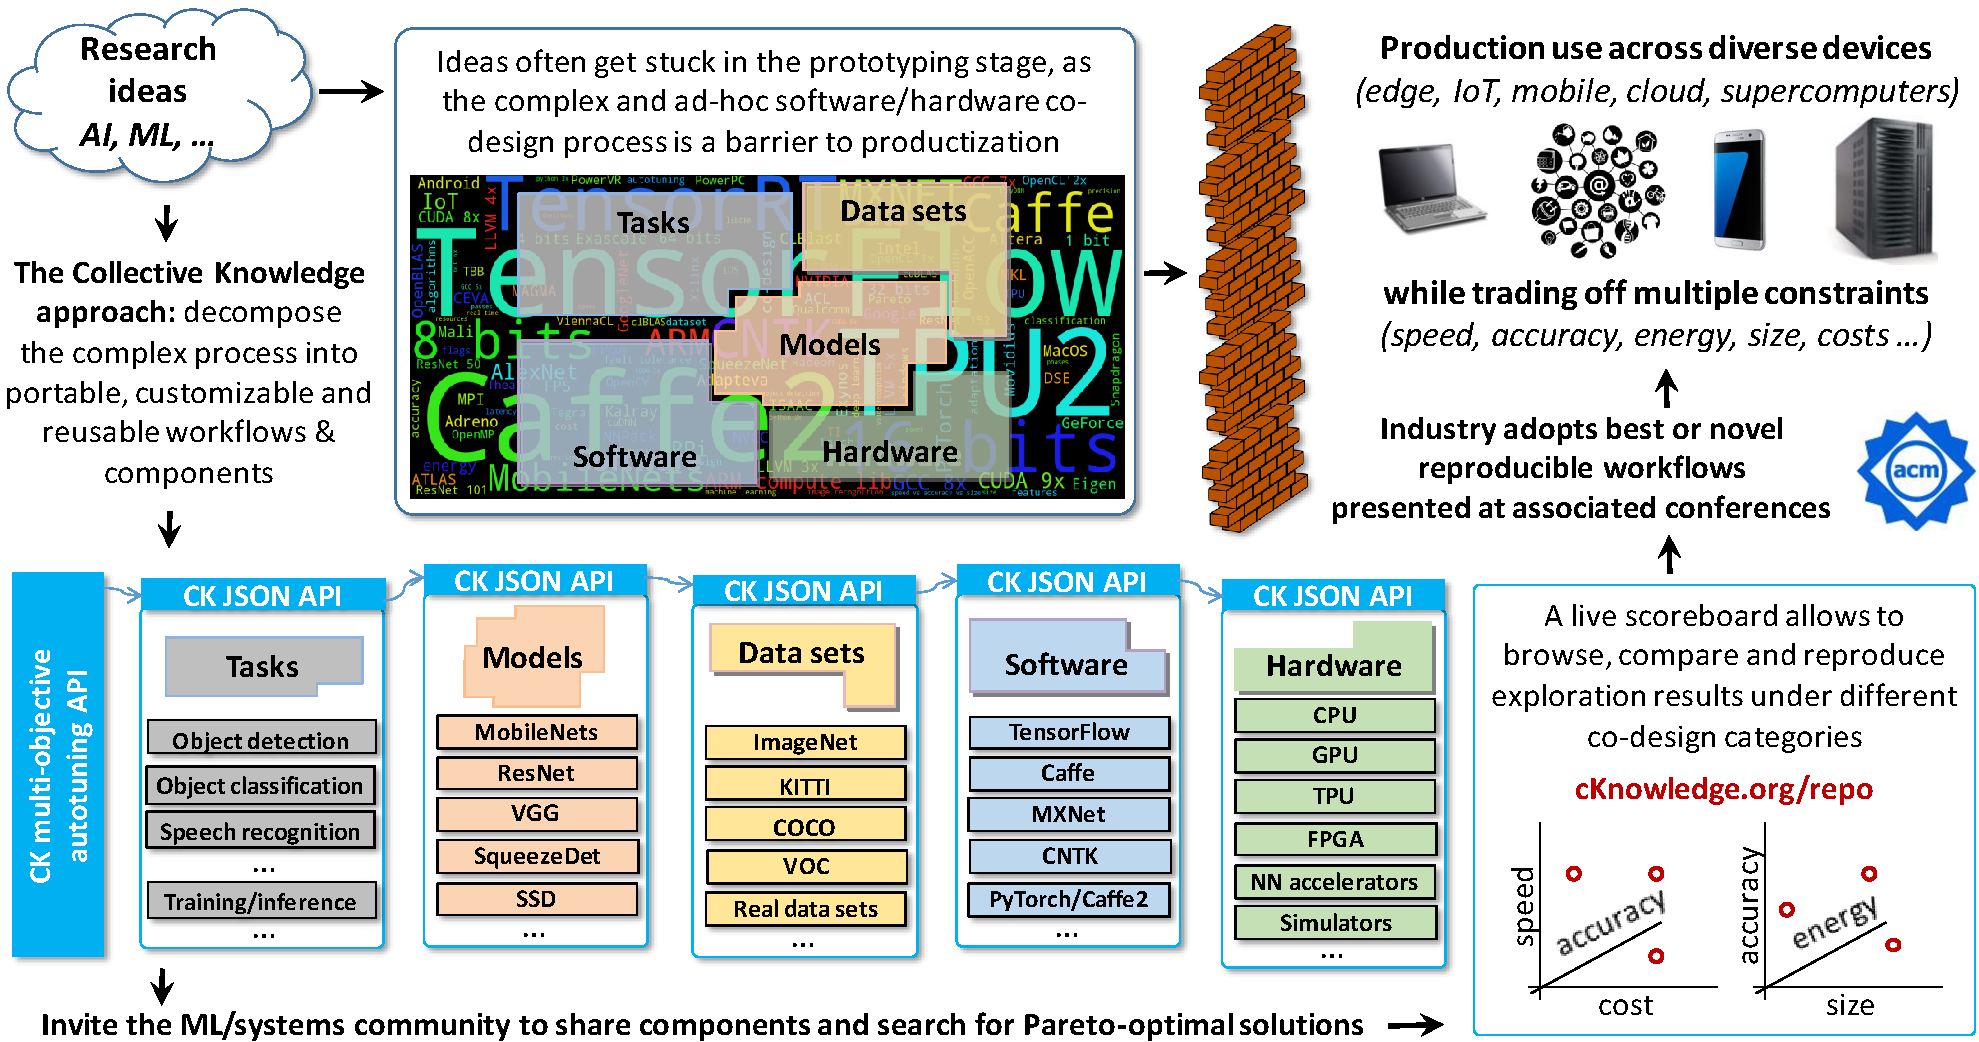
\includegraphics[width=0.9\textwidth]{figures/ck-request-concept-cropped.pdf}
\end{center}

The ReQuEST-ASPLOS'18 proceedings, available in the 
\href{https://dl.acm.org}{ACM Digital Library}, include five papers with Artifact Appendices
and a set of \href{https://www.acm.org/publications/policies/artifact-review-badging}{ACM reproducibility badges}. 
The proceedings are accompanied by snapshots of Collective Knowledge workflows
covering a very diverse model/software/hardware stack:

\begin{packed_itemize}

 \item \textbf{Models:} MobileNets, ResNet-18, ResNet-50, Inception-v3, VGG16, AlexNet, SSD.
 \item \textbf{Data types:} 8-bit integer, 16-bit floating-point (half), 32-bit floating-point (float).
 \item \textbf{AI frameworks and libraries:} MXNet, TensorFlow, Caffe, Keras, Arm Compute Library, cuDNN, TVM, NNVM.
 \item \textbf{Platforms:} Xilinx Pynq-Z1 FPGA, Arm Cortex CPUs and Arm Mali GPGPUs (Linaro HiKey960 and T-Firefly RK3399), a farm of Raspberry Pi devices, NVIDIA Jetson TX1 and TX2, and Intel Xeon servers in Amazon Web Services, Google Cloud and Microsoft Azure.

\end{packed_itemize}

The validated ReQuEST-ASPLOS'18 \href{http://github.com/ctuning/ck-request-asplos18-results}{results}, 
available on the \href{http://cKnowledge.org/request-results}{ReQuEST scoreboard}, also exhibit amazing diversity:

\begin{packed_itemize}

 \item \textbf{Latency:} 4 .. 500 milliseconds per image
 \item \textbf{Throughput:} 2 .. 465 images per second
 \item \textbf{Top 1 accuracy:} 41 .. 75 percent
 \item \textbf{Top 5 accuracy:} 65 .. 93 percent
 \item \textbf{Model size (pre-trained weights):} 2 .. 130 megabytes
 \item \textbf{Peak power consumption:} 2.5 .. 180 Watts
 \item \textbf{Device frequency:} 100 .. 2600 megahertz
 \item \textbf{Device cost:} 40 .. 1200 dollars
 \item \textbf{Cloud usage cost:} 2.6E-6 .. 9.5E-6 dollars per inference

\end{packed_itemize}

Most importantly, the community can now access all the above
CK workflows under permissive licenses and continue
collaborating on them via dedicated 
\href{https://github.com/ctuning/ck-request-asplos18-results}{ReQuEST'18 GitHub projects}. 
First, the workflows can be automatically \href{https://github.com/ctuning/ck/wiki/Portable-workflows}{adapted}
to new platforms and environments by either detecting already
installed dependencies (e.g.\ libraries) or rebuilding
dependencies via an integrated \href{http://cKnowledge.org/shared-packages.html}{package manager} supporting
Linux, Windows, MacOS and Android. Second, the workflows can
be customized by swapping in new models, data sets,
frameworks, libraries, and so on. Third, the workflows can be
extended to expose new design and optimization choices (e.g.\ quantization), as well as evaluation metrics (e.g. power
or memory consumption). Finally, the workflows can be used for
collaborative autotuning ("\href{http://cKnowledge.org/rpi-crowd-tuning}{crowd-tuning}") 
to explore huge optimization spaces using devices such as 
\href{https://play.google.com/store/apps/details?id=openscience.crowdsource.video.experiments}{Android phones and tablets}, 
with best solutions being made available to the
community on the \href{http://cKnowledge.org/dnn-crowd-benchmarking-results}{online CK scoreboard}.

Our overwhelmingly positive experience has also allowed us to
critically assess several potential issues with scaling
up this approach and suggest how to overcome them:

\begin{packed_itemize}

 \item

Fair competitive benchmarking between different platforms,
frameworks and models is hard work. It requires carefully
considering model equivalence (e.g.\ performing the same mix of
operations), input equivalence (e.g.\  preprocessing the inputs
in the same way), output equivalence (e.g.\ validating the
outputs for each input, not just calculating the usual
aggregate accuracy score), etc. Formalizing the benchmarking
requirements and encapsulating them in shared CK components
(e.g.\ using a framework-independent model representation such
as \href{https://onnx.ai/}{ONNX}) and workflows (e.g.\ for input conversion and output
validation), should help standardize and automate the
benchmarking process.

 \item

Thorough artifact evaluation can take several person-weeks.
Each submitted workflow needs to be studied in detail in its
original form and then converted into a common format.
However, the more reusable CK components (such as 
\href{http://cKnowledge.org/shared-programs.html}{workflows},
\href{http://cKnowledge.org/shared-modules.html}{modules/plugins}, 
\href{http://cKnowledge.org/shared-packages.html}{packages}) 
are shared by the community, the easier the conversion becomes. 
For example, we have
successfully reused several previously 
\href{https://github.com/ctuning/ck/wiki#user-content-reusable-ck-components}{shared components} 
for models, frameworks and libraries, as well as the universal
CK workflow for \href{http://cKnowledge.org/rpi-crowd-tuning}{program benchmarking and autotuning}.
We propose to introduce a new 
\href{https://www.acm.org/publications/policies/artifact-review-badging}{ACM reproducibility badge} 
for such unified "plug\&play" components. This could eventually
lead to creating a "marketplace" for Pareto-efficient
implementations (code and data) shared as portable,
customizable and reusable CK components.

%\begin{center}
\includegraphics{ck-assets/artifacts_automated_dl.jpg}\end{center}

 \item

Artifact evaluation may require access to expensive
computational resources (e.g.\ cloud instances with 72-core
servers), proprietary tools (e.g. Intel compilers), and
auxiliary hardware (e.g.\ power meters). Raising the profile
of AE by widely recognizing its benefits and impact should
help us obtain access, licensees and sponsorship from the
industry and funding agencies.

 \item

Full experimental evaluation can take many weeks (for example,
when validating accuracy on 50,000 images on a 100 MHz FPGA
board). The AE committee can collaborate with the authors
to determine a minimally useful scope for evaluation which
would still provide insights to the community. The community
can eventually crowdsource full evaluation. In other words,
AE can be "staged" with a quick check that the artifacts are
"functional" before the camera-ready deadline followed by full
evaluation using the ReQuEST methodology. In fact, ReQuEST can
grow into a non-profit service to conferences and journals.
Sponsorship should help attract experienced full-time
evaluators, as well as part-time volunteers, to work
on unifying and evaluating artifacts and workflows.

\end{packed_itemize}



Our future plans include:

\begin{packed_itemize}

\item collaborating with the community, our Advisory Board and ACM to address the above issues;
\item using the ReQuEST experience to assist AE at the upcoming \href{http://sysml.cc}{SysML'19} conference;
\item replacing non-representative benchmarks with realistic workloads;
\item creating realistic training sets based on mispredictions shared by the community;
\item improving the benchmarking and co-design methodology, and contributing to emerging benchmarking initiatives such as \href{http://mlperf.org}{MLPerf};
\item collaborating with other competitions such as \href{https://rebootingcomputing.ieee.org/lpirc}{LPIRC}, \href{https://dawn.cs.stanford.edu/benchmark}{DAWNBench} and \href{https://sc18.supercomputing.org/experience/studentssc/student-cluster-competition}{SCC} on developing a common experimental framework;
\item standardizing \href{http://cKnowledge.org/rpi-crowd-tuning}{multi-objective autotuning and co-design workflows};
\item improving and documenting the experimental framework and scoreboard;
\item generating reproducible and interactive reports (see examples \href{http://cknowledge.org/repo/web.php?wcid=report:request-overview}{1} and \href{http://cKnowledge.org/rpi-crowd-tuning}{2});
\item adding new shared components such as workloads, data sets, tools and platforms;
\item automating AE "at the source" by integrating CK workflows with e.g.\ \href{https://hotcrp.com/}{HotCRP};
\item standardizing APIs and meta-descriptions of shared components to make them "marketplace-ready";
\item running new ReQuEST competitions for other workloads!

\end{packed_itemize}

We are also organizing a related \href{http://rescue-hpc.org}{ResCuE-HPC workshop}
at \href{https://sc18.supercomputing.org/}{Supercomputing'18} to discuss with the community some of the
above issues focusing on how to develop reproducible,
customizable and portable workflows for high-performance
computing (HPC).

Our long-term vision is to dramatically reduce the complexity
and costs of the development and deployment of AI, ML and
other emerging workloads. We believe that having an open
repository (marketplace) of customizable workflows with
reusable components helps to bring together the
multidisciplinary community to collaboratively co-design,
optimize and autotune computer systems across the full
model/software/hardware stack. Systems integrators will also
benefit from being able to assemble complete solutions
by adapting such reusable components to their specific usage
scenarios, requirements and constraints. We envision that our
community-driven approach and decentralized marketplace will
help accelerate adoption and technology transfer of novel
AI/ML techniques similar to the open-source movement.

%%%%%%%%%%%%%%%%%%%%%%%%%%%%%%%%%%%%%%%%%%%%%%%%%%%%%%%%%%%%%%%%%%%%%%%%%%%%%%%%%%%%%%%%%%%%%%%%%
\section*{Acknowledgments}

We thank the ReQuEST Advisory Board for their enthusiastic
support of our vision; the ReQuEST authors for being very
responsive when converting their workflows to the CK format
and during artifact evaluation; Flavio Vella and Nikolai
Chunosov for their help with unifying and evaluating
submissions; Xipeng Shen and James Tuck for their support for
organizing the ReQuEST workshop at ASPLOS'18; Craig Rodkin,
Asad Ali and Wayne Graves for helping to prepare the ACM DL
proceedings with CK workflows, and the CK community for their
contributions.


%%%%%%%%%%%%%%%%%%%%%%%%%%%%%%%%%%%%%%%%%%%%%%%%%%%%%%%%%%%%%%%%%%%%%%%%%%%%%%%%%%%%%%%%%%%%%%%%%
\section*{Organizers (A-Z)}

\begin{packed_itemize}

 \item Luis Ceze, University of Washington, USA
 \item Natalie Enright Jerger, University of Toronto, Canada
 \item Babak Falsafi, EPFL, Switzerland
 \item \textit{Grigori Fursin, cTuning foundation, France (reproducibility and common workflow framework)}
 \item \textit{Anton Lokhmotov, dividiti, UK (industrial relations)}
 \item \textit{Thierry Moreau, University of Washington, USA (workshop organization)}
 \item Adrian Sampson, Cornell University, USA
 \item Phillip Stanley Marbell, University of Cambridge, UK 

\end{packed_itemize}

%%%%%%%%%%%%%%%%%%%%%%%%%%%%%%%%%%%%%%%%%%%%%%%%%%%%%%%%%%%%%%%%%%%%%%%%%%%%%%%%%%%%%%%%%%%%%%%%%
\section*{Advisory board (A-Z)}

\begin{packed_itemize}

 \item Michaela Blott, Xilinx
 \item Unmesh Bordoloi, General Motors
 \item Ofer Dekel, Microsoft
 \item Maria Girone, CERN openlab
 \item Wayne Graves, ACM
 \item Vinod Grover, NVIDIA
 \item Sumit Gupta, IBM
 \item James Hetherington, Alan Turing Institute
 \item Steve Keckler, NVIDIA
 \item Wei Li, Intel
 \item Colin Osborne, Arm
 \item Andrew Putnam, Microsoft
 \item Boris Shulkin, Magna
 \item Greg Stoner, AMD
 \item Alex Wade, Chan Zuckerberg Initiative
 \item Peng Wu, Huawei
 \item Cliff Young, Google 

\end{packed_itemize}

%%%%%%%%%%%%%%%%%%%%%%%%%%%%%%%%%%%%%%%%%%%%%%%%%%%%%%%%%%%%%%%%%%%%%%%%%%%%%%%%%%%%%%%%%%%%%%%%%
\section*{Table of contents}
\label{sec:overview}

\begin{tabular}{|p{2.85in}|p{0.52in}|p{0.62in}|p{0.56in}|p{0.69in}|p{0.63in}|}
\hline\hline
  \begin{center}\small\textbf{Paper}\end{center} &   \begin{center}\small\textbf{Artifact\newline available}\end{center} &   \begin{center}\small\textbf{Artifact\newline functional}\end{center} &   \begin{center}\small\textbf{Artifact\newline reusable}\end{center} &   \begin{center}\small\textbf{Results\newline reproduced}\end{center} &   \begin{center}\small\textbf{Results\newline replicated}\end{center} \\
\hline
  \textbf{Highly Efficient 8-bit Low Precision Inference of Convolutional Neural Networks with IntelCaffe}\newline\newline{Jiong Gong, Haihao Shen, Guoming Zhang, Xiaoli Liu, Shane Li, Ge Jin, Niharika Maheshwari, Evarist Fomenko, Eden Segal}\newline\newline [~\href{https://doi.org/10.1145/3229762.3229763}{Paper DOI}~] [~\href{https://doi.org/10.1145/3229769}{Artifact DOI}~] [~\href{https://github.com/intel/caffe}{Original artifact}~] [~\href{https://github.com/ctuning/ck-request-asplos18-caffe-intel}{CK workflow}~] [~\href{https://github.com/ctuning/ck-request-asplos18-results-caffe-intel}{CK results}~]\newline &  \begin{center}
\includegraphics{ck-assets/artifacts_available_dl.jpg}\end{center} &  ~ &  \begin{center}
\includegraphics{ck-assets/artifacts_evaluated_reusable_dl.jpg}\end{center} &  ~ &  \begin{center}
\includegraphics{ck-assets/results_replicated_dl.jpg}\end{center} \\
\hline
  \textbf{Optimizing Deep Learning Workloads on Arm GPU with TVM}\newline\newline{Lianmin Zheng, Tianqi Chen}\newline\newline [~\href{https://doi.org/10.1145/3229762.3229764}{Paper DOI}~] [~\href{https://doi.org/10.1145/3229770}{Artifact DOI}~] [~\href{https://github.com/merrymercy/tvm-mali}{Original artifact}~] [~\href{https://github.com/ctuning/ck-request-asplos18-mobilenets-tvm-arm}{CK workflow}~] [~\href{https://github.com/ctuning/ck-request-asplos18-results-mobilenets-tvm-arm}{CK results}~]\newline &  \begin{center}
\includegraphics{ck-assets/artifacts_available_dl.jpg}\end{center} &  ~ &  \begin{center}
\includegraphics{ck-assets/artifacts_evaluated_reusable_dl.jpg}\end{center} &  ~ &  \begin{center}
\includegraphics{ck-assets/results_replicated_dl.jpg}\end{center} \\
\hline
  \textbf{Real-Time Image Recognition Using Collaborative IoT Devices}\newline\newline{Ramyad Hadidi, Jiashen Cao, Matthew Woodward, Michael S. Ryoo, Hyesoon Kim}\newline\newline [~\href{https://doi.org/10.1145/3229762.3229765}{Paper DOI}~] [~\href{https://doi.org/10.1145/3229771}{Artifact DOI}~] [~\href{https://github.com/parallel-ml/asplos2018-workshop}{Original artifact}~] [~\href{https://github.com/ctuning/ck-request-asplos18-iot-farm}{CK workflow}~] [~\href{https://github.com/ctuning/ck-request-asplos18-results-iot-farm}{CK results}~]\newline &  \begin{center}
\includegraphics{ck-assets/artifacts_available_dl.jpg}\end{center} &  ~ &  \begin{center}
\includegraphics{ck-assets/artifacts_evaluated_reusable_dl.jpg}\end{center} &  ~ &  \begin{center}
\includegraphics{ck-assets/results_replicated_dl.jpg}\end{center} \\
\hline
  \textbf{Leveraging the VTA-TVM Hardware-Software Stack for FPGA Acceleration of 8-bit ResNet-18 Inference}\newline\newline{Thierry Moreau}\newline\newline [~\href{https://doi.org/10.1145/3229762.3229766}{Paper DOI}~] [~\href{https://doi.org/10.1145/3229772}{Artifact DOI}~] [~\href{https://github.com/uwsaml/vta}{Original artifact}~] [~\href{https://github.com/ctuning/ck-request-asplos18-resnet-tvm-fpga}{CK workflow}~] [~\href{https://github.com/ctuning/ck-request-asplos18-results-resnet-tvm-fpga}{CK results}~]\newline &  ~ &  \begin{center}
\includegraphics{ck-assets/artifacts_evaluated_functional_dl.jpg}\end{center} &  ~ &  ~ &  \begin{center}
\includegraphics{ck-assets/results_replicated_dl.jpg}\end{center} \\
\hline
  \textbf{Multi-objective autotuning of MobileNets across the full software/hardware stack}\newline\newline{Anton Lokhmotov, Nikolay Chunosov, Flavio Vella, Grigori Fursin}\newline\newline [~\href{https://doi.org/10.1145/3229762.3229767}{Paper DOI}~] [~\href{https://doi.org/10.1145/3229773}{Artifact DOI}~] [~\href{https://github.com/dividiti/ck-request-asplos18-mobilenets-armcl-opencl}{CK workflow}~] [~\href{https://github.com/ctuning/ck-request-asplos18-results-mobilenets-armcl-opencl}{CK results}~]\newline &  \begin{center}
\includegraphics{ck-assets/artifacts_available_dl.jpg}\end{center} &  ~ &  \begin{center}
\includegraphics{ck-assets/artifacts_evaluated_reusable_dl.jpg}\end{center} &  ~ &  \begin{center}
\includegraphics{ck-assets/results_replicated_dl.jpg}\end{center} \\
\hline
\hline
\end{tabular}

\end{document}
